% Options for packages loaded elsewhere
\PassOptionsToPackage{unicode}{hyperref}
\PassOptionsToPackage{hyphens}{url}
\PassOptionsToPackage{dvipsnames,svgnames,x11names}{xcolor}
%
\documentclass[
  letterpaper,
  DIV=11,
  numbers=noendperiod]{scrartcl}

\usepackage{amsmath,amssymb}
\usepackage{lmodern}
\usepackage{iftex}
\ifPDFTeX
  \usepackage[T1]{fontenc}
  \usepackage[utf8]{inputenc}
  \usepackage{textcomp} % provide euro and other symbols
\else % if luatex or xetex
  \usepackage{unicode-math}
  \defaultfontfeatures{Scale=MatchLowercase}
  \defaultfontfeatures[\rmfamily]{Ligatures=TeX,Scale=1}
\fi
% Use upquote if available, for straight quotes in verbatim environments
\IfFileExists{upquote.sty}{\usepackage{upquote}}{}
\IfFileExists{microtype.sty}{% use microtype if available
  \usepackage[]{microtype}
  \UseMicrotypeSet[protrusion]{basicmath} % disable protrusion for tt fonts
}{}
\makeatletter
\@ifundefined{KOMAClassName}{% if non-KOMA class
  \IfFileExists{parskip.sty}{%
    \usepackage{parskip}
  }{% else
    \setlength{\parindent}{0pt}
    \setlength{\parskip}{6pt plus 2pt minus 1pt}}
}{% if KOMA class
  \KOMAoptions{parskip=half}}
\makeatother
\usepackage{xcolor}
\usepackage[top=1in,right=.8in,bottom=1in,left=.8in]{geometry}
\setlength{\emergencystretch}{3em} % prevent overfull lines
\setcounter{secnumdepth}{-\maxdimen} % remove section numbering
% Make \paragraph and \subparagraph free-standing
\ifx\paragraph\undefined\else
  \let\oldparagraph\paragraph
  \renewcommand{\paragraph}[1]{\oldparagraph{#1}\mbox{}}
\fi
\ifx\subparagraph\undefined\else
  \let\oldsubparagraph\subparagraph
  \renewcommand{\subparagraph}[1]{\oldsubparagraph{#1}\mbox{}}
\fi

\usepackage{color}
\usepackage{fancyvrb}
\newcommand{\VerbBar}{|}
\newcommand{\VERB}{\Verb[commandchars=\\\{\}]}
\DefineVerbatimEnvironment{Highlighting}{Verbatim}{commandchars=\\\{\}}
% Add ',fontsize=\small' for more characters per line
\usepackage{framed}
\definecolor{shadecolor}{RGB}{241,243,245}
\newenvironment{Shaded}{\begin{snugshade}}{\end{snugshade}}
\newcommand{\AlertTok}[1]{\textcolor[rgb]{0.68,0.00,0.00}{#1}}
\newcommand{\AnnotationTok}[1]{\textcolor[rgb]{0.37,0.37,0.37}{#1}}
\newcommand{\AttributeTok}[1]{\textcolor[rgb]{0.40,0.45,0.13}{#1}}
\newcommand{\BaseNTok}[1]{\textcolor[rgb]{0.68,0.00,0.00}{#1}}
\newcommand{\BuiltInTok}[1]{\textcolor[rgb]{0.00,0.23,0.31}{#1}}
\newcommand{\CharTok}[1]{\textcolor[rgb]{0.13,0.47,0.30}{#1}}
\newcommand{\CommentTok}[1]{\textcolor[rgb]{0.37,0.37,0.37}{#1}}
\newcommand{\CommentVarTok}[1]{\textcolor[rgb]{0.37,0.37,0.37}{\textit{#1}}}
\newcommand{\ConstantTok}[1]{\textcolor[rgb]{0.56,0.35,0.01}{#1}}
\newcommand{\ControlFlowTok}[1]{\textcolor[rgb]{0.00,0.23,0.31}{#1}}
\newcommand{\DataTypeTok}[1]{\textcolor[rgb]{0.68,0.00,0.00}{#1}}
\newcommand{\DecValTok}[1]{\textcolor[rgb]{0.68,0.00,0.00}{#1}}
\newcommand{\DocumentationTok}[1]{\textcolor[rgb]{0.37,0.37,0.37}{\textit{#1}}}
\newcommand{\ErrorTok}[1]{\textcolor[rgb]{0.68,0.00,0.00}{#1}}
\newcommand{\ExtensionTok}[1]{\textcolor[rgb]{0.00,0.23,0.31}{#1}}
\newcommand{\FloatTok}[1]{\textcolor[rgb]{0.68,0.00,0.00}{#1}}
\newcommand{\FunctionTok}[1]{\textcolor[rgb]{0.28,0.35,0.67}{#1}}
\newcommand{\ImportTok}[1]{\textcolor[rgb]{0.00,0.46,0.62}{#1}}
\newcommand{\InformationTok}[1]{\textcolor[rgb]{0.37,0.37,0.37}{#1}}
\newcommand{\KeywordTok}[1]{\textcolor[rgb]{0.00,0.23,0.31}{#1}}
\newcommand{\NormalTok}[1]{\textcolor[rgb]{0.00,0.23,0.31}{#1}}
\newcommand{\OperatorTok}[1]{\textcolor[rgb]{0.37,0.37,0.37}{#1}}
\newcommand{\OtherTok}[1]{\textcolor[rgb]{0.00,0.23,0.31}{#1}}
\newcommand{\PreprocessorTok}[1]{\textcolor[rgb]{0.68,0.00,0.00}{#1}}
\newcommand{\RegionMarkerTok}[1]{\textcolor[rgb]{0.00,0.23,0.31}{#1}}
\newcommand{\SpecialCharTok}[1]{\textcolor[rgb]{0.37,0.37,0.37}{#1}}
\newcommand{\SpecialStringTok}[1]{\textcolor[rgb]{0.13,0.47,0.30}{#1}}
\newcommand{\StringTok}[1]{\textcolor[rgb]{0.13,0.47,0.30}{#1}}
\newcommand{\VariableTok}[1]{\textcolor[rgb]{0.07,0.07,0.07}{#1}}
\newcommand{\VerbatimStringTok}[1]{\textcolor[rgb]{0.13,0.47,0.30}{#1}}
\newcommand{\WarningTok}[1]{\textcolor[rgb]{0.37,0.37,0.37}{\textit{#1}}}

\providecommand{\tightlist}{%
  \setlength{\itemsep}{0pt}\setlength{\parskip}{0pt}}\usepackage{longtable,booktabs,array}
\usepackage{calc} % for calculating minipage widths
% Correct order of tables after \paragraph or \subparagraph
\usepackage{etoolbox}
\makeatletter
\patchcmd\longtable{\par}{\if@noskipsec\mbox{}\fi\par}{}{}
\makeatother
% Allow footnotes in longtable head/foot
\IfFileExists{footnotehyper.sty}{\usepackage{footnotehyper}}{\usepackage{footnote}}
\makesavenoteenv{longtable}
\usepackage{graphicx}
\makeatletter
\def\maxwidth{\ifdim\Gin@nat@width>\linewidth\linewidth\else\Gin@nat@width\fi}
\def\maxheight{\ifdim\Gin@nat@height>\textheight\textheight\else\Gin@nat@height\fi}
\makeatother
% Scale images if necessary, so that they will not overflow the page
% margins by default, and it is still possible to overwrite the defaults
% using explicit options in \includegraphics[width, height, ...]{}
\setkeys{Gin}{width=\maxwidth,height=\maxheight,keepaspectratio}
% Set default figure placement to htbp
\makeatletter
\def\fps@figure{htbp}
\makeatother

\usepackage{fancyhdr}
\usepackage{titling}
\pagestyle{fancy}
\fancyhf{}
\renewcommand\maketitle{
  \fancyhead[C]{
    \thetitle
    \ifx \theauthor\empty  \else \ – \theauthor \fi
    \ifx \thedate\empty  \else \ – \thedate \ \fi
  }
}
\fancyfoot[C]{\thepage}
\KOMAoption{captions}{tableheading,figureheading}
\makeatletter
\makeatother
\makeatletter
\makeatother
\makeatletter
\@ifpackageloaded{caption}{}{\usepackage{caption}}
\AtBeginDocument{%
\ifdefined\contentsname
  \renewcommand*\contentsname{Table of contents}
\else
  \newcommand\contentsname{Table of contents}
\fi
\ifdefined\listfigurename
  \renewcommand*\listfigurename{List of Figures}
\else
  \newcommand\listfigurename{List of Figures}
\fi
\ifdefined\listtablename
  \renewcommand*\listtablename{List of Tables}
\else
  \newcommand\listtablename{List of Tables}
\fi
\ifdefined\figurename
  \renewcommand*\figurename{Figure}
\else
  \newcommand\figurename{Figure}
\fi
\ifdefined\tablename
  \renewcommand*\tablename{Table}
\else
  \newcommand\tablename{Table}
\fi
}
\@ifpackageloaded{float}{}{\usepackage{float}}
\floatstyle{ruled}
\@ifundefined{c@chapter}{\newfloat{codelisting}{h}{lop}}{\newfloat{codelisting}{h}{lop}[chapter]}
\floatname{codelisting}{Listing}
\newcommand*\listoflistings{\listof{codelisting}{List of Listings}}
\makeatother
\makeatletter
\@ifpackageloaded{caption}{}{\usepackage{caption}}
\@ifpackageloaded{subcaption}{}{\usepackage{subcaption}}
\makeatother
\makeatletter
\@ifpackageloaded{tcolorbox}{}{\usepackage[many]{tcolorbox}}
\makeatother
\makeatletter
\@ifundefined{shadecolor}{\definecolor{shadecolor}{rgb}{.97, .97, .97}}
\makeatother
\makeatletter
\makeatother
\ifLuaTeX
  \usepackage{selnolig}  % disable illegal ligatures
\fi
\IfFileExists{bookmark.sty}{\usepackage{bookmark}}{\usepackage{hyperref}}
\IfFileExists{xurl.sty}{\usepackage{xurl}}{} % add URL line breaks if available
\urlstyle{same} % disable monospaced font for URLs
\hypersetup{
  pdftitle={Assignment 4: Sensitivity Analysis},
  pdfauthor={Guillermo Romero},
  colorlinks=true,
  linkcolor={blue},
  filecolor={Maroon},
  citecolor={Blue},
  urlcolor={Blue},
  pdfcreator={LaTeX via pandoc}}

\title{Assignment 4: Sensitivity Analysis}
\author{Guillermo Romero}
\date{5/9/23}

\begin{document}
\maketitle
\ifdefined\Shaded\renewenvironment{Shaded}{\begin{tcolorbox}[frame hidden, boxrule=0pt, breakable, sharp corners, borderline west={3pt}{0pt}{shadecolor}, enhanced, interior hidden]}{\end{tcolorbox}}\fi

For a given forest, you will perform a sensitivity analysis of model
predictions of conductance Consider the sensitivity of your estimate to
uncertainty in the following parameters and inputs • height • kd • k0 •
v

Windspeeds v are normally distributed with a mean of 250 cm/s with a
standard deviation of 30 cm/s

For vegetation height assume that height is somewhere between 9.5 and
10.5 m (but any value in that range is equally likely)

For the kd and k0 parameters you can assume that they are normally
distributed with standard deviation of 1\% of their default values

\hypertarget{a}{%
\subsubsection{a)}\label{a}}

Use the Latin hypercube approach to generate parameter values for the 4
parameters

\begin{Shaded}
\begin{Highlighting}[]
\FunctionTok{source}\NormalTok{(}\StringTok{"Catm{-}1.R"}\NormalTok{)}
\end{Highlighting}
\end{Shaded}

\begin{Shaded}
\begin{Highlighting}[]
\CommentTok{\# set a random seed to make things \textquotesingle{}random\textquotesingle{}}
\FunctionTok{set.seed}\NormalTok{(}\DecValTok{42}\NormalTok{)}

\CommentTok{\# specify parameters}
\NormalTok{pnames }\OtherTok{=} \FunctionTok{c}\NormalTok{(}\StringTok{"v"}\NormalTok{, }\StringTok{"height"}\NormalTok{,}\StringTok{"k\_o"}\NormalTok{, }\StringTok{"k\_d"}\NormalTok{)}

\CommentTok{\# how many parameters}
\NormalTok{npar }\OtherTok{=}  \FunctionTok{length}\NormalTok{(pnames)}
               
\CommentTok{\# how many samples}
\NormalTok{nsample }\OtherTok{=} \DecValTok{50}

\CommentTok{\# random values array matrix using LHS for the parameters}
\NormalTok{parm\_quant }\OtherTok{=} \FunctionTok{randomLHS}\NormalTok{(nsample, npar)}
\FunctionTok{colnames}\NormalTok{(parm\_quant) }\OtherTok{=}\NormalTok{ pnames}


\NormalTok{parm }\OtherTok{=} \FunctionTok{as.data.frame}\NormalTok{(}\FunctionTok{matrix}\NormalTok{(}\AttributeTok{nrow=}\FunctionTok{nrow}\NormalTok{(parm\_quant), }\AttributeTok{ncol=}\FunctionTok{ncol}\NormalTok{(parm\_quant)))}
\FunctionTok{colnames}\NormalTok{(parm) }\OtherTok{=}\NormalTok{ pnames}



\NormalTok{parm[,}\StringTok{"v"}\NormalTok{] }\OtherTok{=} \FunctionTok{qnorm}\NormalTok{(parm\_quant[,}\StringTok{"v"}\NormalTok{], }\AttributeTok{mean=}\DecValTok{250}\NormalTok{, }\AttributeTok{sd=}\DecValTok{30}\NormalTok{)}

\NormalTok{parm[,}\StringTok{"k\_d"}\NormalTok{] }\OtherTok{=} \FunctionTok{qnorm}\NormalTok{(parm\_quant[,}\StringTok{"k\_d"}\NormalTok{], }\AttributeTok{mean=}\FloatTok{0.7}\NormalTok{, }\AttributeTok{sd=}\NormalTok{.}\DecValTok{007}\NormalTok{)}

\NormalTok{parm[,}\StringTok{"k\_o"}\NormalTok{] }\OtherTok{=} \FunctionTok{qnorm}\NormalTok{(parm\_quant[,}\StringTok{"k\_o"}\NormalTok{], }\AttributeTok{mean=}\FloatTok{0.1}\NormalTok{, }\AttributeTok{sd=}\NormalTok{.}\DecValTok{001}\NormalTok{)}

\CommentTok{\# uniform}
\NormalTok{parm[,}\StringTok{"height"}\NormalTok{] }\OtherTok{=} \FunctionTok{qunif}\NormalTok{(parm\_quant[,}\StringTok{"height"}\NormalTok{], }\AttributeTok{min =} \FloatTok{9.5}\NormalTok{, }\AttributeTok{max =} \FloatTok{10.5}\NormalTok{)}
\end{Highlighting}
\end{Shaded}

\hypertarget{b}{%
\subsubsection{b)}\label{b}}

Run the atmospheric conductance model for these parameters

\begin{Shaded}
\begin{Highlighting}[]
\NormalTok{Ca\_outputs }\OtherTok{=} \FunctionTok{pmap}\NormalTok{(parm, Catm)}

\CommentTok{\# Use map\_dfr to create param\_outputs dataframe}
\NormalTok{parameter\_outputs }\OtherTok{\textless{}{-}} \FunctionTok{map\_dfr}\NormalTok{(}\FunctionTok{seq\_along}\NormalTok{(Ca\_outputs), }\SpecialCharTok{\textasciitilde{}}\NormalTok{parm[.x,] }\SpecialCharTok{\%\textgreater{}\%} \FunctionTok{mutate}\NormalTok{(}\AttributeTok{output =}\NormalTok{ Ca\_outputs[[.x]]))}
\end{Highlighting}
\end{Shaded}

\#c) Plot conductance estimates in a way that accounts for parameter
uncertainty

\begin{Shaded}
\begin{Highlighting}[]
\FunctionTok{ggthemr}\NormalTok{(}\StringTok{\textquotesingle{}flat dark\textquotesingle{}}\NormalTok{, }\AttributeTok{type =}\StringTok{\textquotesingle{}outer\textquotesingle{}}\NormalTok{, }\AttributeTok{layout=} \StringTok{\textquotesingle{}minimal\textquotesingle{}}\NormalTok{)}

\NormalTok{tmp }\OtherTok{=}\NormalTok{ parameter\_outputs }\SpecialCharTok{\%\textgreater{}\%} \FunctionTok{gather}\NormalTok{(pnames, }\AttributeTok{key=}\StringTok{"parameter"}\NormalTok{, }\AttributeTok{value=}\StringTok{"value"}\NormalTok{)}
\FunctionTok{ggplot}\NormalTok{(tmp, }\FunctionTok{aes}\NormalTok{(}\AttributeTok{x =}\NormalTok{ parameter, }\AttributeTok{y =}\NormalTok{ value, }\AttributeTok{col =}\NormalTok{ parameter)) }\SpecialCharTok{+}
  \FunctionTok{geom\_boxplot}\NormalTok{() }\SpecialCharTok{+}
  \FunctionTok{labs}\NormalTok{(}\AttributeTok{y =} \StringTok{"Parameter Value"}\NormalTok{, }\AttributeTok{title =} \StringTok{"Boxplot of Parameters"}\NormalTok{)}
\end{Highlighting}
\end{Shaded}

\begin{figure}[H]

{\centering 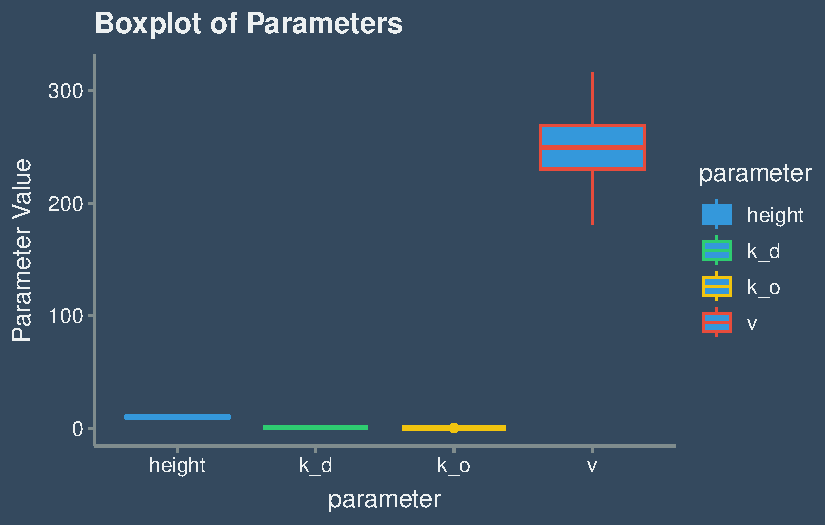
\includegraphics{sensitivity-analysis_files/figure-pdf/unnamed-chunk-5-1.pdf}

}

\end{figure}

\begin{Shaded}
\begin{Highlighting}[]
\CommentTok{\# Graph the cumulative distribution}
\FunctionTok{ggplot}\NormalTok{(parameter\_outputs, }\FunctionTok{aes}\NormalTok{(output)) }\SpecialCharTok{+}
  \FunctionTok{stat\_ecdf}\NormalTok{() }\SpecialCharTok{+}
  \FunctionTok{labs}\NormalTok{(}\AttributeTok{x =} \StringTok{"Conductance Estimates"}\NormalTok{, }\AttributeTok{y =} \StringTok{"Cumulative Distribution"}\NormalTok{, }\AttributeTok{title =} \StringTok{"Cumulative Distribution of Conductance Estimates"}\NormalTok{) }
\end{Highlighting}
\end{Shaded}

\begin{figure}[H]

{\centering 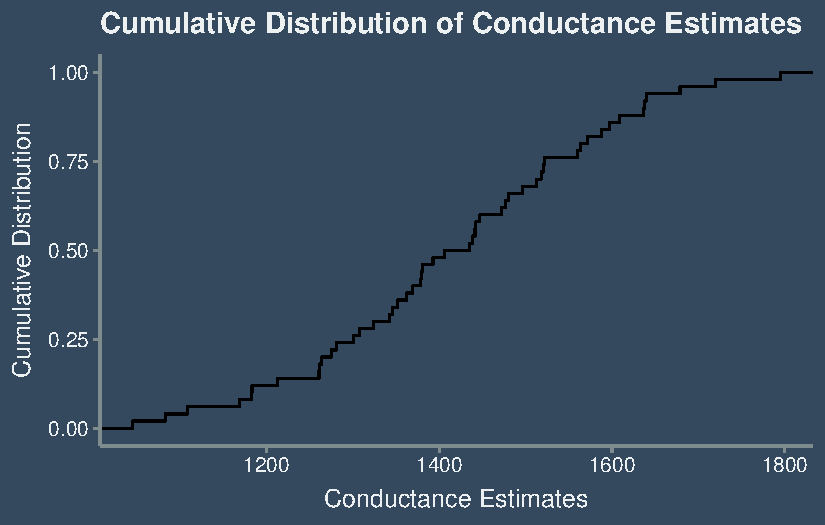
\includegraphics{sensitivity-analysis_files/figure-pdf/unnamed-chunk-6-1.pdf}

}

\end{figure}

\hypertarget{d}{%
\subsubsection{d)}\label{d}}

Plot conductance estimates against each of your parameters

\begin{Shaded}
\begin{Highlighting}[]
\CommentTok{\# Create plots for parameters effect on output}

\NormalTok{parameter\_outputs }\SpecialCharTok{|\textgreater{}} 
  \FunctionTok{pivot\_longer}\NormalTok{(}\AttributeTok{cols =}\NormalTok{ v}\SpecialCharTok{:}\NormalTok{k\_d, }\AttributeTok{names\_to =} \StringTok{"parm"}\NormalTok{, }\AttributeTok{values\_to =} \StringTok{"value"}\NormalTok{) }\SpecialCharTok{|\textgreater{}} 
  \FunctionTok{ggplot}\NormalTok{( }\FunctionTok{aes}\NormalTok{(}\AttributeTok{x =}\NormalTok{ value, }\AttributeTok{y =}\NormalTok{ output, }\AttributeTok{col =}\NormalTok{ parm)) }\SpecialCharTok{+}
  \FunctionTok{geom\_point}\NormalTok{(}\AttributeTok{size =} \FloatTok{1.5}\NormalTok{) }\SpecialCharTok{+}
  \FunctionTok{facet\_wrap}\NormalTok{(}\SpecialCharTok{\textasciitilde{}}\NormalTok{ parm, }\AttributeTok{ncol =} \DecValTok{2}\NormalTok{, }\AttributeTok{scales =} \StringTok{"free"}\NormalTok{) }
\end{Highlighting}
\end{Shaded}

\begin{figure}[H]

{\centering 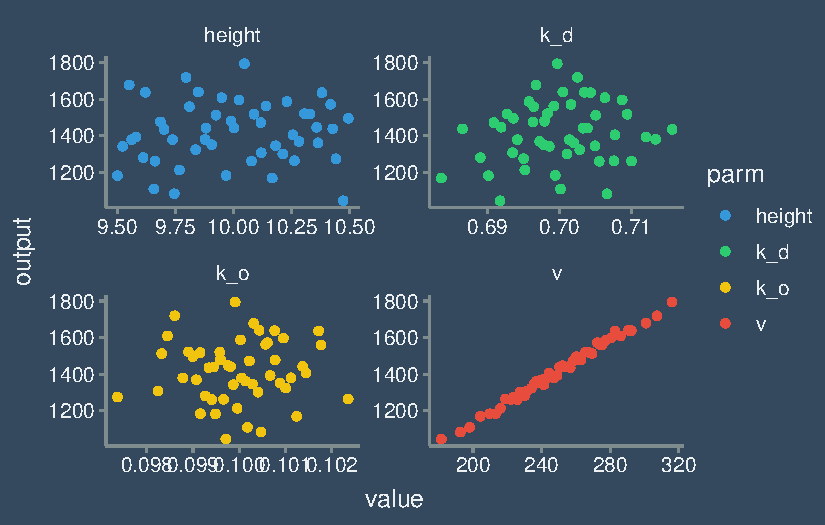
\includegraphics{sensitivity-analysis_files/figure-pdf/unnamed-chunk-7-1.pdf}

}

\end{figure}

\begin{Shaded}
\begin{Highlighting}[]
  \FunctionTok{labs}\NormalTok{(}\AttributeTok{x =} \StringTok{"Value"}\NormalTok{, }\AttributeTok{y =} \StringTok{"Output"}\NormalTok{, }\AttributeTok{color =} \StringTok{"Parameter"}\NormalTok{, }\AttributeTok{title =} \StringTok{"Ca Model Output by Parameter"}\NormalTok{)}
\end{Highlighting}
\end{Shaded}

\begin{verbatim}
$x
[1] "Value"

$y
[1] "Output"

$colour
[1] "Parameter"

$title
[1] "Ca Model Output by Parameter"

attr(,"class")
[1] "labels"
\end{verbatim}

\hypertarget{e}{%
\subsubsection{e)}\label{e}}

Estimate the Partial Rank Correlation Coefficients

\begin{Shaded}
\begin{Highlighting}[]
\NormalTok{partial\_correlation }\OtherTok{=} \FunctionTok{pcc}\NormalTok{(parm, parameter\_outputs}\SpecialCharTok{$}\NormalTok{output, }\AttributeTok{rank =} \ConstantTok{TRUE}\NormalTok{)}

\FunctionTok{plot}\NormalTok{(partial\_correlation)}
\end{Highlighting}
\end{Shaded}

\begin{figure}[H]

{\centering 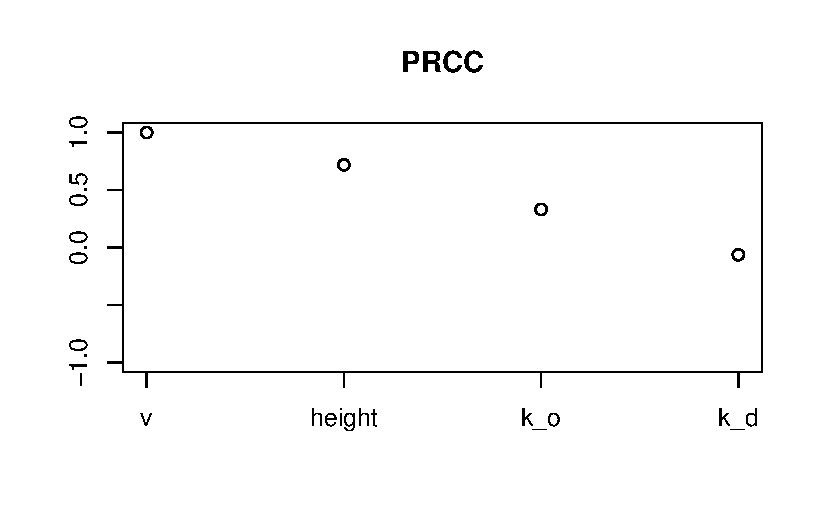
\includegraphics{sensitivity-analysis_files/figure-pdf/unnamed-chunk-8-1.pdf}

}

\end{figure}

\hypertarget{f}{%
\subsubsection{f)}\label{f}}

Discuss what your results tell you about how aerodynamic conductance?
What does it suggest about what you should focus on if you want to
reduce uncertainty in aerodymaic conductance estimates? Does this tell
you anything about the sensitivity of plant water use to climate change?

\textbf{The results indicate that aerodynamic conductance is highly
sensitive to windspeed. To reduce uncertainty in conductance estimates,
focus on minimizing windspeed variability. This suggests that climate
change, by potentially affecting windspeed, could influence plant water
use through its impact on conductance.}



\end{document}
